\documentclass{article}

\usepackage[utf8]{inputenc}
% \usepackage[latin1]{inputenc}
\usepackage[ngerman,naustrian]{babel}
\usepackage{lmodern}
\usepackage[T1]{fontenc}
\usepackage{ulem}
\usepackage{here}
\usepackage[pdftex]{graphicx}
\usepackage{amsthm}
\usepackage{gensymb}
\usepackage{fancyhdr}
\usepackage[left=20mm,top=25mm,bottom=25mm,right=20mm,headheight=15mm,headsep=10mm,footskip=10mm]{geometry}
\usepackage{longtable}
\usepackage{hhline}
\usepackage[table]{xcolor}
\usepackage{amsfonts}
\usepackage{amssymb}
\usepackage{amsmath}
\usepackage{mathcomp}
\usepackage{tabularx}
\usepackage{multicol}
\usepackage{graphicx}
\renewcommand{\familydefault}{\sfdefault}
		% \sffamily

\newcommand{\bild}[3]{\begin{figure}[h!]		\begin{center}			\includegraphics[#3]{#1}			\caption{#2}		\end{center}	\end{figure}}

\begin{document}

%\pagestyle{empty}
\begin{titlepage}
	\begin{center}
		{\large{FH OÖ - Hagenberg \\ embedded systems design}\\\vspace*{4cm}}
		\small{RTO1 UE}\\
		\textbf{WS 2020}\\\vspace*{2cm}
		\Huge{\textbf{Protokoll}}\\\vspace*{1cm}
		\huge{Übung\,1: Vorversion von Betriebssystemen\\ \large{kooperative Weitergabe an Tasks } } \vspace*{90mm}
		
		\small{Simon Steindl  S2010567025	\\
		Florian Hinterleitner S2010567014	\\
		}
	\end{center}
\end{titlepage}

% \tableofcontents
% \newpage
% \setcounter{page}{18}
% \setcounter{section}{3}
 
\section{Übungsaufgabe A – Erstellung einer Debug-Unit}
% screenshots
% Timing-tabelle

\subsection{Debug-Unit}
% 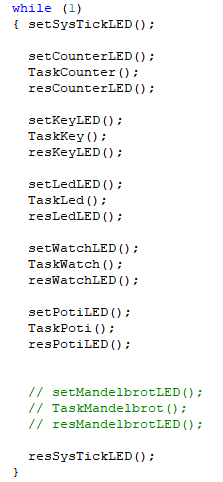
\includegraphics[width=.8\textwidth]{debugUnit}
	\begin{figure}[h!]
		\begin{center}
			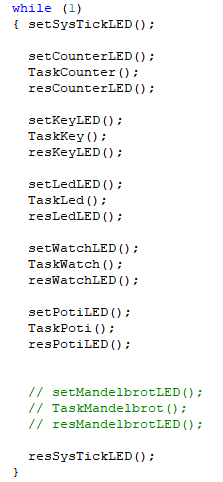
\includegraphics{debugUnit}
			\caption{mit deaktivierter Mandelbrot-Sektion}
		\end{center}
	\end{figure}

-  Messen Sie die Laufzeit jedes Tasks \\

	\begin{table}[h!]
		\begin{center}		
			\begin{tabular}{ l | l }	 % \hline
				Task & Laufzeit in ms \\ \hline
				Systick mit Mandelbrot	& 18.52s \\ \hline
				Systick ohne Mandelbrot	& 29.39 	\\ \hline
				Systick ohne GPIOs *)	& 29.38 \\ \hline
				Counter	& 6.135 \\ \hline
				Key& 4.895 \\ \hline
				LED	& 4.894 \\ \hline
				Watch	& 7.346 \\ \hline
				Poti	& 6.115 \\ \hline
				Mandelbrot	& 18.49s \\ %\hline
			\end{tabular}
			\caption{Laufzeiten des SysTicks, sowie der einzelnen Tasks}
		\end{center}		
	\end{table}

		

	*) jedoch mit SysTick GPIOs, ohne die gar keine Messung möglich wäre
	
\subsection{Ergebnisse}
\subsection{Laufzeit jedes Tasks}
\subsection{ Screenshots der Messungen }

	\begin{figure}[h!]
		\begin{center}
			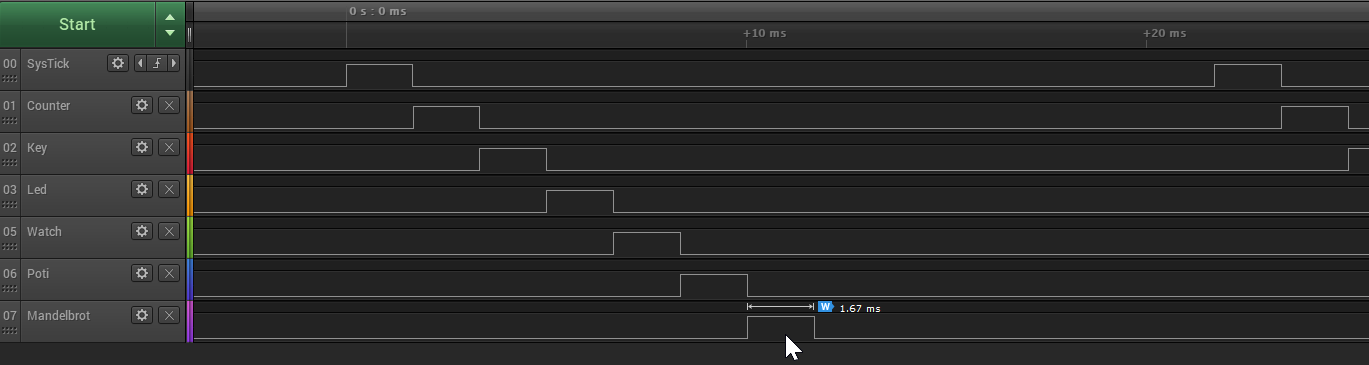
\includegraphics[width=.8\textwidth]{tryGPIO}
			\caption{GPIO-Treppe zum korrekten Verkabeln und Zuordnen der LA-Kanäle zu Tasks}
		\end{center}
	\end{figure}


\bild{02_mitMandelbrot}{mitMandelbrot}{width=\textwidth}
\bild{03_ohneMandelbrot_time}{ohneMandelbrot timed}{width=\textwidth}
\bild{03_ohneMandelbrot}{ohneMandelbrot}{width=\textwidth}

\subsection{Overhead (Zyklen, µs) der Messung}
-  Geben Sie an, wie viel Overhead (Zyklen, µs) der Code der Messung verursacht \\
	1 sleep() mit 10000 NOPs entspricht 1.67ms (1.668ms) \\
	Systick 31.86ms ohne allem
	33.10ms mit allen LEDS

\section{Übungsaufgabe B – Reaktionsgeschwindigkeit bei Superloops}
\ldots


\end{document} 